\section{Asynchronous Many-task Runtime Systems}
A parallel programming model includes a programming  model, which refers to the mechanism for a program to express the concurrency, and an execution model, indicating how the program creates and controls concurrency\cite{kulkarni2019comparative, bennett2015asynchronous}.
Some of the common existing execution models include fork-join, Communicating Sequential Processes(CSP), event-based models and actor model\cite{bennett2015asynchronous}. 
Some of the current parallel programming frameworks include, accelerator-based programming models like OpenACC\cite{wienke2012openacc}, OpenCL\cite{munshi2009opencl}, and CUDA\cite{nvidia2011nvidia}, shared-memory programming models like Intel TBB\cite{reinders2007intel}, Cilk\cite{blumofe1996cilk}, OpenMP\cite{dagum1998openmp}, and distributed-memory programming models like MPI\cite{mpi1994message}, Charm++\cite{kale1993charm++}, Parallex\cite{kaiser2009parallex}, UPC\cite{kulkarni2019comparative}.

A runtime system is in charge of creating and managing the concurrency, through implementing parts of an execution model\cite{bennett2015asynchronous}.
An asynchronous many-task(AMT) model on the other hand, is a category of programming model and execution model. 
An AMT programming model breaks the work into small and transferable tasks along with their associated input. In an AMT execution model, tasks are being executed when their inputs are available rather than in a well defined order\cite{bennett2015asynchronous}. 

Some of well known AMT runtimes include: HPX\cite{kaiser2014hpx}, Charm++\cite{kale1993charm++}, Uintah\cite{germain2000uintah}, Legion\cite{bauer2012legion}.

\vspace{\baselineskip}
\subsection{HPX}
HPX\cite{kaiser2014hpx} is a C++ runtime system for parallel and distributed applications based on ParalleX execution model\cite{kaiser2009parallex}. 
%HPX contains 5 main modules: Performance Monitoring System, Local Control Objects(LCOs), Thread Scheduling System, Parcel Transport Layer, Active Global Address Space (AGAS)\cite{kaiser2009parallex}.
HPX provides you with lightweight user-level threads with fast context switching\cite{kulkarni2019comparative}. Whenever one thread is blocked, the scheduler picks a ready thread based on a scheduling policy. This allows you to hide the latency, and avoid starvation while keeping a high utilization of the resources\cite{kulkarni2019comparative}.  

\vspace{\baselineskip}
\subsubsection{Execution Model}
The "SLOW" model identifies four potential sources for performance degradation as: Starvation, Latency, Overheads, and Waiting or contention\cite{kaiser2009parallex}.

Starvation refers to a situation where there is insufficient amount work for the computing resource. this could be due to insufficient total amount of work available, or unbalanced distribution of work among resources\cite{kulkarni2019comparative}. 

Latency is the time distance, usually measured in processor clock, of accessing remote data or services\cite{gao2007parallex}.  

Overhead refers to the effort that needs to be taken to manage parallel resources and actions on the critical path\cite{kulkarni2019comparative}.

Finally, waiting is the contention of the shared physical and logical resources causing one request to be blocked by another access of the same resource\cite{gao2007parallex}. This could happen due to limited network bandwidth, shared communication channels, memory bank conflicts\cite{kulkarni2019comparative},\cite{gao2007parallex}. 


\vspace{\baselineskip}
\section{Blaze}
Blaze Math Library\cite{iglberger2012expression} is a C++ library for linear algebra. Blaze, based upon Expression Templates(ETs)\cite{veldhuizen1995expression}, introduces "smart" expression templates(SETs)\cite{iglberger2012expression} to optimize the performance for array-based operations. Expression Templates\cite{veldhuizen1995expression} is an abstraction technique that uses overloaded operators in C++ to prevent creation of unnecessary temporaries, while evaluating arithmetic expressions, in order to improve the performance\cite{iglberger2012expression}. The ET-based approaches create a parse tree of the expression at compile time and postpone the actual evaluation to when the expression is assigned to a target. 

Although being able to achieve promising performances for element-wise operations, these methods are not suitable for high performance computing for the following reasons. Due to their abstraction from both the data type and also the operation itself, they do not allow optimizations specific to the type of the arrays, alongside the operation\cite{iglberger2012expression}. As a solution, Blaze proposes smart ETs with these three main additions: integration with architecture-specific highly optimized compute kernels, creation of intermediate temporaries when needed, and selecting optimal evaluation method automatically for compound expressions\cite{iglberger2012expression}. 

Some of the ET-based linear algebra libraries are: Blitz++\cite{Blitz}, Boost uBLAS\cite{ublas}, MTL\cite{MTL}, and Eigen\cite{guennebaud2010eigen}. Among these libraries, Eigen, MTL, alongside Blaze, impose different conceptual changes to ETs in order to make them suitable for HPC.    
Blaze also makes it possible for programmers to utilize SIMD(Single Instruction Multiple Data) vectorization simply by adding a compile time flag.

\vspace{\baselineskip}
\section{Task Granularity}\label{task}
Defining the grain size as the amount of work assigned to one HPX thread, Grubel\cite{grubel2015performance} studies the effect of grain size on the execution time for a fixed number of cores. The results show that, for small grain sizes the overhead of creating the tasks, and for large grain sizes the starvation, is the dominant factor affecting the execution time\cite{grubel2015performance}. When grain size is small, to perform same amount of work, higher number of tasks is created, and there is an overhead associated with creation of each task. Although this overhead is very small (order of microseconds), when the amount of work performed by each thread is also small, this overhead becomes significant. A the grain size increases, these overheads are amortized by the time it takes to execute the task. 

On the other hand, when grain size is increases, the number of tasks being created decreases, up until a point where the number of tasks being created is smaller than the number of cores. At this point another factor would interfere with the performance, which is referred to as starvation. Starvation happens where a large amount of work is assigned to some of the cores while the other cores are idling. At this point we are not using our resources efficiently. 

While overheads of creating tasks degrades the performance for small grain sizes and starvation causes the execution time to increase for large grain sizes, there is a region in between where changing the grain size does not affect the performance. 

\vspace{\baselineskip}
\begin{figure}[H]
	\centering
	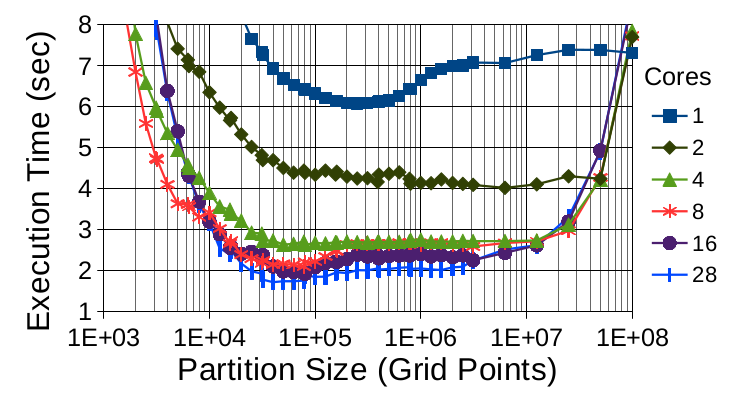
\includegraphics[scale=0.6]{images/task_granularity.png}
	\caption{The effect of task size on execution time for Stencil application \cite{grubel2015performance}}	
	\label{fig_task_gran}
\end{figure}

%\vspace{\baselineskip}
%\section{Modeling performance}
%Gunther states the factors involved in creating overheads as, exchanging data between memory and processors, waiting for completion of a memory access or an I/O, 
%\begin{itemize}
%	\item 
%	\item
%\end{itemize}



\vspace{\baselineskip}
\section{Universal Scalibility Law}
Amdahl's law\cite{amdahl1967validity}, states that the amount of achievable speed up by adding more processors when running a parallel application, is restricted by the amount of code that could actually be parallelized. 
Equation \ref{Amdahl}, shows the relationship between speedup and number of processors, where $\sigma$ is the serial fraction of the execution time, based on Amdahl's law\cite{gunther2007guerrilla}. 

\begin{equation}\label{Amdahl}
S(p) = \frac{p}{1+\sigma(p-1)}\\
\end{equation}

On the other hand, Gunther\cite{gunther2007guerrilla} extends Amdahl's law by incorporating the effect of three factors, namely concurrency, contention, and coherency, as shown in Equation~\ref{USL}.

\begin{equation}\label{USL}
S(p) = \frac{p}{1+\sigma(p-1)+\kappa{p}(p-1)}\\
\end{equation}

Concurrency($p$) represents the linear speedup that could have been achieved if no interaction existed among the processors, contention($\sigma$) represents the serialization effect of shared writable data, and finally coherency or data consistency($\kappa$) represents the effort that needs to be made for keeping shared writable data consistent\cite{gunther2007guerrilla}.    

Figure~\ref{fig_Amdahl} shows an example of the ideal linear speedup we expect to see when increasing the number of the processors, against the actual achievable speedup based on Amdahl's law and USL.

Equation~\ref{USL_generalized} generalizes Equation~\ref{USL} to represent the throughput by adding another parameter($\gamma$) to represent the serial throughput.

\begin{equation}\label{USL_generalized}
X(p) = \frac{\gamma{p}}{1+\sigma(p-1)+\kappa{p}(p-1)}\\
\end{equation}

\begin{figure}[H]
	\centering
	\includegraphics[scale=0.8]{images/Amdahls.png}
	\caption{An example of the achievable speedup based on Amdahl's law and USL compared to the ideal linear speedup where $\sigma=0.04$ and $\kappa=0.005$.}	
	\label{fig_Amdahl}
\end{figure}

Universal scalibility law also suggests that for some values of $\sigma$ and $\kappa$ there could be a certain number of processors that yield to maximum performance\cite{gunther2007guerrilla}. Increasing the number of processor beyond that point would only cause performance degradation.  

\vspace{\baselineskip}
\subsection{Other Models}	
There are a few other models that have also been suggested to simulate the scalibility. Geometric model is a one-parameter model, in which speedup has the following relationship with the number of processors:
\begin{equation}\label{geo}
S(p) = \frac{1-\phi^{p}}{1-\phi}\\
\end{equation}

The parameter $\phi$, where $0<\phi\leqslant1$, is called the MP factor, and it represents the remaining section of the processor capacity after deducting overheads. 
The geometric model is nonphysical for large number of processors, due to inconsistency with Coxian queuing model\cite{gunther2002new}. 

Quadratic model\cite{gunther2000practical}, with overhead parameter $\gamma$, where $0	\leqslant\gamma<1$, is represented in Equation{quad}.
\begin{equation}\label{quad}
S(p) = p-\gamma{p(p-1)}\\
\end{equation}

The quadratic model has a critical point at: 
\begin{equation}\label{quad_critical}
p^* = \lfloor\frac{1+\gamma}{2\gamma}\rfloor \\
\end{equation}

The problem with this model is that its not physical. This model represents an inverted parabola that will intersect the x axis at two points, implying that there with be a certain number of processors starting from which the speedup would be negative. 


Exponential model, is also a single parameter model $\alpha$ where $0<\alpha\leqslant1$. This parameter is a combination of coherency and contention. 

\begin{equation}\label{expo}
S(p) = p(1-\alpha)^{(p-1)}\\
\end{equation}

This model also has a critical point, but this point is very sensitive to $\alpha$. Although this model works very well for small number of processors, it imposes a severe capacity degradation for large number of processors.

\vspace{\baselineskip}
\section{Loop Scheduling}
Loop scheduling refers to different ways iterations could be assigned to the processors and the order of their execution. 
The main reason for performance degradation in loop scheduling is load imbalance, which refers to situations where different amount of work is assigned to different processors\cite{ciorba2018openmp}.    

The simplest loop scheduling method is static scheduling, in which, the iterations are divided evenly among all the processors statically, either as a consecutive block -also called cyclic- or in a round-robin manner\cite{liu1994safe}. Since all the assignments happen at compile time or before execution of the application, this method imposes no runtime scheduling overhead. Several factors including interprocessor communication, cache misses, and page faults can lead to different execution times for different iterations, leading to load imbalance among the processors\cite{philip1995increasing}.

In the meanwhile, dynamic scheduling methods postpone the assignment to runtime, which tends to improve load balancing, at the cost of higher scheduling overhead. Some of dynamic scheduling methods include: Pure Self-scheduling, Chunk Self-scheduling, Guided Self-scheduling\cite{polychronopoulos1987guided}, Factoring\cite{hummel1992factoring} and Trapazoid Self-scheduling\cite{tzen1993trapezoid},\cite{liu1994safe}.We briefly go over some of these loop scheduling techniques here.


In Pure Self-scheduling every time a processors becomes idle, it fetches one loop iteration. This approach, while achieving a high load balance, imposes a considerable amount of scheduling overhead when we are dealing with a fine-grain workload, and a large number of iterations. Also frequent access to shared variables like loop index could lead to memory contention\cite{liu1994safe}. 

In order to decrease the high scheduling overhead of Pure Self-scheduling methods, Chunk Self-scheduling method assigns a certain number of iterations(called chunk size) to each idle processor. This method trades lower scheduling overhead with higher load imbalance. Selection of the chunk size plays a very important role in the performance, as so a large chunk size increases the scheduling overhead decreases and causes load imbalance, while a small chunk size increases memory contention and scheduling overhead\cite{liu1994safe}. 

As an adaptive loop scheduling technique, Guided Self-scheduling\cite{polychronopoulos1987guided} divides the remaining number of iterations at each request evenly among the processors, and assigns it to the processor that made the request, while updating the number of remaining iterations. This causes larger number of iterations to be assigned to the processors at the beginning of the loop execution, which results in lower scheduling overhead. The number of iterations assigned to each processor decreases as it approaches to the end of the execution, generating tasks containing only one or two iterations, causing an increase in the scheduling overhead. In order to tackle this issue, a minimum number of chunks could be set to avoid creation of very small chunks\cite{lilja1994exploiting}. 

Very similar to Guided Self-scheduling, Factoring\cite{hummel1992factoring} also decreases the chunk size as the loop execution proceeds, with this difference that it does it in batches of equal sized chunks. If the first iterations of the loop are more time consuming then the rest of the iterations, Factoring performs better than Guided scheduling\cite{mohammed2018experimental}.  


Along with the mentioned loop scheduling approaches, two other scheduling techniques can be utilized for load balancing. Work stealing\cite{blumofe1999scheduling} lets the processors to steal work from other processors queue, resulting in a more balanced load distribution. In work sharing on the other hand, each time a processor creates new threads, the scheduler would try to migrate some of them to other processors for a more balanced lad distribution\cite{blumofe1999scheduling}.



But each of these methods work well for specific problem. We are looking for a general solution which can automatically decide on the chunk size parameter to achieve the best performance.

\vspace{\baselineskip}	